%Solución del Ejercicio 2 por medio de la metodología 6D

\subsection{Descripción del problema}
 Dada una ecuación cuadrática regresar los valores de las raíces en caso de que estén sobre el conjunto de los números reales, en caso contrario indicar que la solución esta en el conjunto de los números complejos.

\begin {figure}[ht]
\centerline{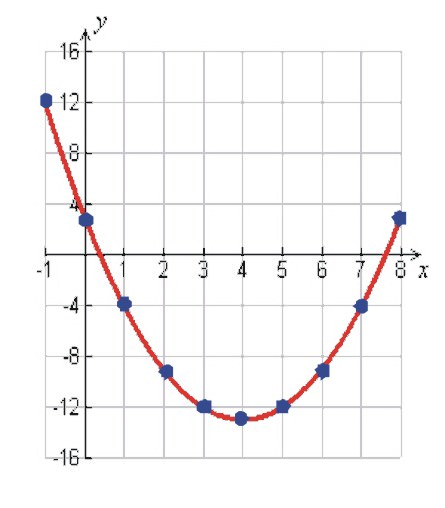
\includegraphics[width = 6cm]{Latex-imágenes/ecuacionC.jpeg}}
\caption{Gráfica de la ecuación cuadrática}
\label{fig}
\end {figure}

\subsection{Definición del problema}
Primero, tenemos que verificar que la ecuación esté en la forma estándar:

\begin{equation}
    ax^2 + bx + c = 0
\end{equation}


donde $a$, $b$ y $c$ son coeficientes reales y $x$ es la variable desconocida. Posteriormente, se deben identificar los valores de $a$, $b$ y $c$ en la ecuación. A continuación, se debe utilizar la fórmula cuadrática para encontrar las soluciones: 
\begin{equation}
x = \frac{-b \pm \sqrt{b^2 - 4ac}}{2a}
\end{equation}


Posteriormente, se sustituyen los valores de $a$, $b$ y $c$ en la fórmula cuadrática y se realizan los cálculos necesarios.\\

\subsection{Diseño de la solución}

Se realizó una representación gráfica de un algoritmo para resolver el problema
\begin {figure}[h!]
\centerline{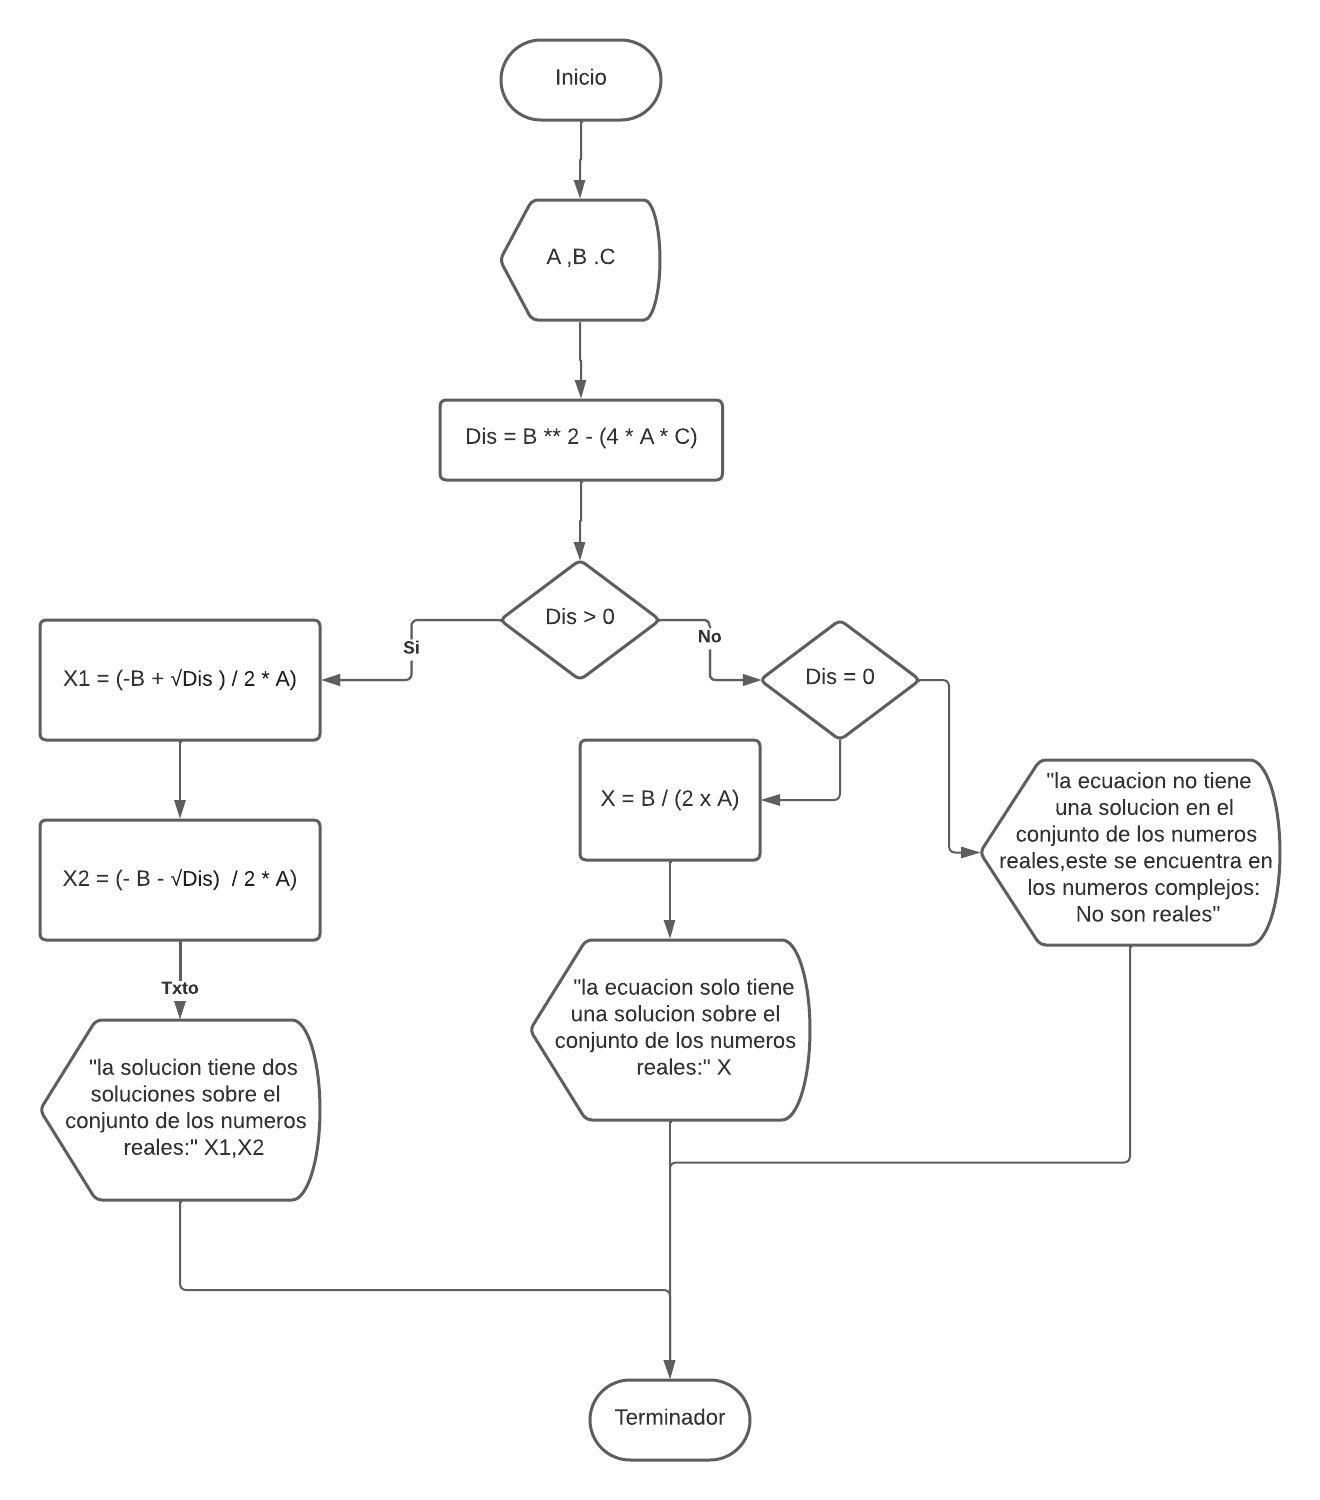
\includegraphics[width = 6cm]{Latex-imágenes/diagramaEx2.jpeg}}
\caption{Diagrama de flujo problema 2.}
\label{fig}
\end {figure}

\subsection{Desarrollo de la solución}
Para solucionar este problema tendrá que resolver los tres coeficientes de los tres parámetros de una ecuación cuadrática que se tenga, donde se desarrollara primero el discriminante y después se evaluara el mismo para determinar si hay dos soluciones, una solución o si todo es falso, no existe, para ello se implemento Este código que solicita al usuario que ingrese los coeficientes de la ecuación cuadrática $a$ $b$ $c$. 
 
\begin{javaCode}

    float a = Float.parseFloat(JOptionPane.
    showInputDialog("Ingresa coeficiente respecto al parámetro \"a\""));
        float b = Float.parseFloat(JOptionPane.
        showInputDialog("Ingresa coeficiente respecto al parámetro \"b\""));
        float c = Float.parseFloat(JOptionPane.
        showInputDialog("Ingresa coeficiente respecto al parámetro \"c\""));
        
\end{javaCode}

posterior a lo que hicimos se va a calcula el discriminante con la ecuación cuadrática.

\begin{javaCode}
  
     double discriminante = Math.pow(b, 2) - (4 * a * c);

\end{javaCode}
 

Para finalizar la discriminante pasa por la primer condición donde se obtendrán dos soluciones, la segunda solución solo nos dará una solución, en caso diferente no hay solución posible.

\begin{javaCode}
 
 if (discriminante > 0) {
            double x1 = (-b + Math.sqrt(discriminante)) / (2 * a);
            double x2 = (-b - Math.sqrt(discriminante)) / (2 * a);

            JOptionPane.showMessageDialog(null, "La solución tiene dos soluciones sobre el conjunto de los números reales:\n" +
                    "x1 = " + x1 + "\n" +
                    "x2 = " + x2);
        } else {
            if (discriminante == 0) {
                double x = -b / (2 * a);
                JOptionPane.showMessageDialog(null, "La ecuación solo tiene una solución sobre el conjunto de los números reales:\n" +
                        "x = " + x);

    
\end{javaCode}

 


\subsection{Depuración de pruebas}

\begin{table}[!ht]
\label{T:equipos}
\begin{center}
\begin{tabular}{| p{.5cm} | p{.5cm} | p{.5cm} | p{5cm} |}
\hline
\textbf{$a$} & \textbf{$b$} & \textbf{$c$} & \textbf{$x_1, x_2$ o $x$}\\
\hline
2 & 10 & 2 & -0.20, -4.79 \\
7 & 8 & 9 & "La ecuación no tiene una solución en el conjunto de los números reales, este se encuentra en los números complejos." \\
-5 & 6 & -1 & 0.2, 1.0 \\
3 & 464 & 46 & "La ecuación no tiene una solución en el conjunto de los números reales, este se encuentra en los números complejos." \\
1 & -4 & 4 & 2 \\
\hline
\end{tabular}
\caption{Tabla de corridas.}
\end{center}
\end{table}
